\chapter{负反馈放大电路的设计与仿真}%
\label{cha:负反馈放大电路的设计与仿真}

\section{实验目的}%
\label{sec:\arabic{chapter}实验目的}

\begin{enumerate}
	\item 设计一个阻容耦合两级电压放大电路,要求信号源频率\SI{20}{\kHz}(峰值\SI{1}{\mV}),负载电阻\SI{20}{\kohm},电压增益大于100;
	\item 给电路引入电压串联负反馈:
		\begin{enumerate}
			\item 测试负反馈接入前后电路放大倍数、输入、输出电阻和频率特性;
			\item 改变输入信号幅度,观察负反馈对电路非线性失真的影响。
		\end{enumerate}
\end{enumerate}

\section{实验要求}%
\label{sec:\arabic{chapter}实验要求}

\begin{Exercise}
	给出引入电压串联负反馈电路的实验接线图。
\end{Exercise}

\begin{Answer}
	电压串联负反馈电路实验接线图见图\ref{fig:两级闭环放大电路}。
\end{Answer}

\begin{Exercise}
	给出负反馈接入前后电路的放大倍数、输入电阻、输出电阻,并验证$ A_\mathrm{F}\approx\dfrac{1}{F} $。
\end{Exercise}

\begin{Answer}
	负反馈接入前后电路的参数见表\ref{tab:反馈前后指标变化},验证见章节\ref{ssub:放大倍数}。
\end{Answer}

\begin{Exercise}
	给出负反馈接入前后电路的频率特性和$ f_\mathrm{L} $、$ f_\mathrm{H} $值,以及输出开始出现失真时的输入信号幅度。
\end{Exercise}

\begin{Answer}
	负反馈接入前后电路的参数和输出开始出现失真时的输入信号幅度见表\ref{tab:反馈前后指标变化}。
\end{Answer}

\begin{Exercise}
	分析实验结果。
\end{Exercise}

\begin{Answer}
	分析见章节\ref{sec:\arabic{chapter}实验小结}。
\end{Answer}

\section{实验步骤}%
\label{sec:\arabic{chapter}实验步骤}

\subsection{设计电路}%
\label{sub:\arabic{chapter}设计电路}

如图\ref{fig:两级开环放大电路}所示即为两级放大电路且无反馈的原理图。

\begin{figure}[H]
	\centering
	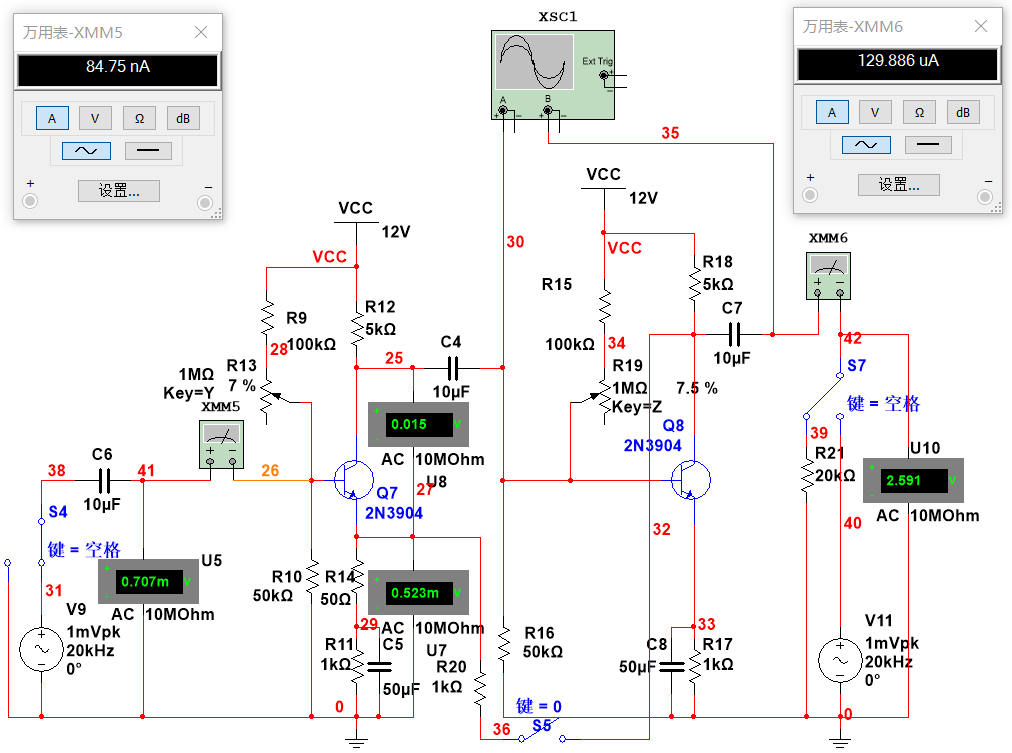
\includegraphics[width = 0.8\linewidth]{3/Ri-open.png}
	\caption{两级开环放大电路}
	\label{fig:两级开环放大电路}
\end{figure}

与单级放大电路类似,采用分压式偏置电路,有效稳定静态工作点。其中$ R_{10},R_9,R_{13} $为第一级电路偏置电阻,$ V_\mathrm{be} = \dfrac{R_{10}}{R9 + R_{13}}V_\mathrm{cc} $,通过调节$ R_{10} $阻值大小可以改变$ V_\mathrm{be} $进而改变静态工作点;$ R_{15}, R_{19}, R_{16} $为第二级电路偏置电阻,$ V_\mathrm{be} = \dfrac{R_{15}}{R_6 + R_{11}}V_\mathrm{cc} $,通过调节$ R_{11} $阻值大小可以改变$ V_\mathrm{be} $进而改变静态工作点;

其中电路放大倍数为第一级、第二级放大倍数之积,为了保证输出信号不失真,因此在第一级电路中加上电阻$ R_{14} $减小第一级放大倍数。由于$ R_{14} $在发射极上,因此交流通路中会阻值等于放大倍数乘以$ R_{14} $,大大减小放大倍数,因此$ R_{14} $不能过大。

如图\ref{fig:两级闭环放大电路}所示即为两级放大电路且有反馈的原理图。

\begin{figure}[H]
	\centering
	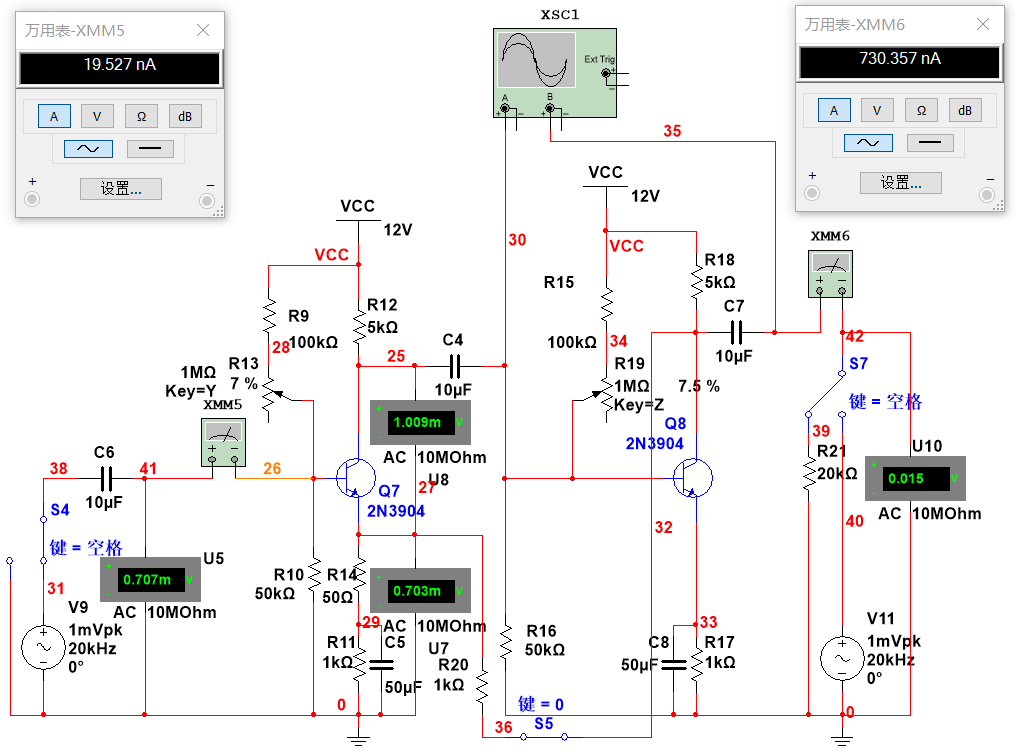
\includegraphics[width = 0.8\linewidth]{3/Ri-close.png}
	\caption{两级闭环放大电路}
	\label{fig:两级闭环放大电路}
\end{figure}

其中反馈电阻为$ R_{20} $,采用电压串联负反馈的方式。为了引入深度负反馈,一般$ R_{20} $阻值为发射极总阻值之和左右。

深度负反馈的主要标志是电路净输入量为0,因此只需测量$ V_\mathrm{b} $、$ V_\mathrm{e} $电压,两者数值相近即$ V_\mathrm{be} $输入量近似为零。

\subsection{指标计算}%
\label{sub:\arabic{chapter}指标计算}

\begin{table}[H]
	\centering
	\caption{两级放大电路参数}
	\label{tab:两级放大电路参数}
	\csvautobooktabular{tab/3/3-1.csv}
\end{table}

\begin{table}[H]
	\centering
	\caption{反馈前后指标变化}
	\label{tab:反馈前后指标变化}
	\csvautobooktabular{tab/3/3-2.csv}
\end{table}

\subsection{仿真结果}%
\label{sub:\arabic{chapter}仿真结果}

\subsubsection{两级放大电路输入电阻}%
\label{ssub:两级放大电路输入电阻}

输入电阻测量原理图如图\ref{fig:两级闭环放大电路}所示,即断开负载电阻,在输入端加入信号源。

采用交流分析法测量输入电阻,由图\ref{fig:两级开环放大电路}可知无反馈时输入电阻为\SI{8.342}{\kohm}。

比较反馈接入前后输入电阻的变化可知电压串联负反馈增大了输入电阻,有利于电路从电压源中获得更大的电压输入,提高电源效率。

\subsubsection{两级放大电路输出电阻}%
\label{ssub:两级放大电路输出电阻}

\begin{figure}[H]
	\centering
	\begin{subfigure}[H]{.7\linewidth}
		\centering
		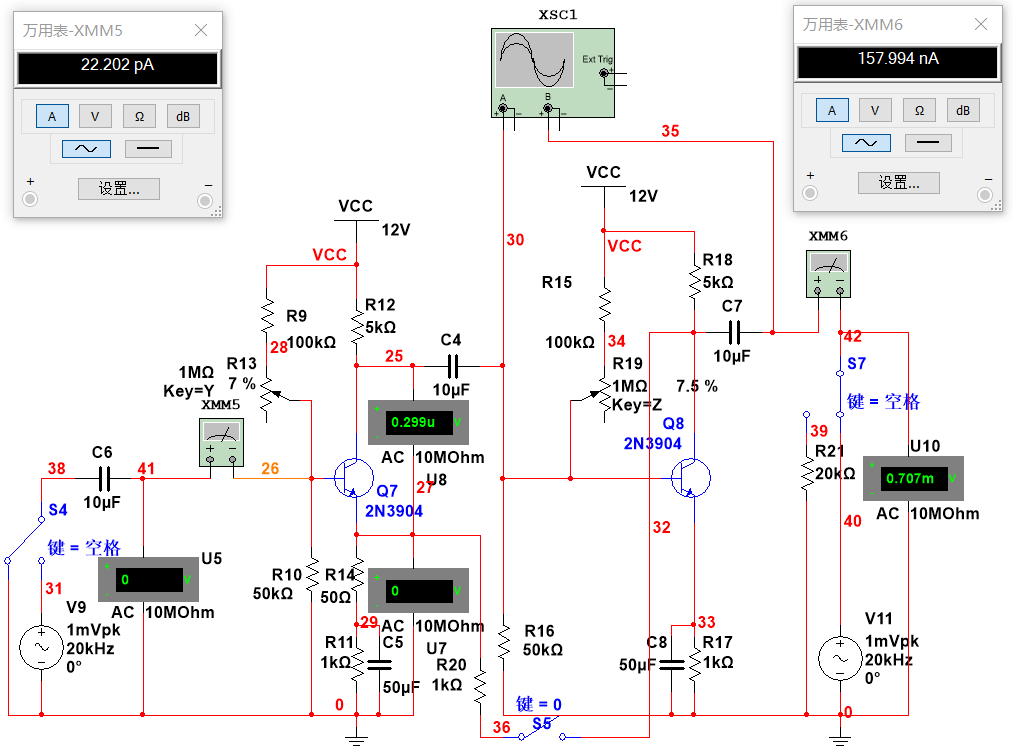
\includegraphics[width=\linewidth]{3/Ro-open.png}
		\caption{两级开环放大电路输出电阻}
		\label{fig:两级开环放大电路输出电阻}
	\end{subfigure}
	\quad
	\begin{subfigure}[H]{.7\linewidth}
		\centering
		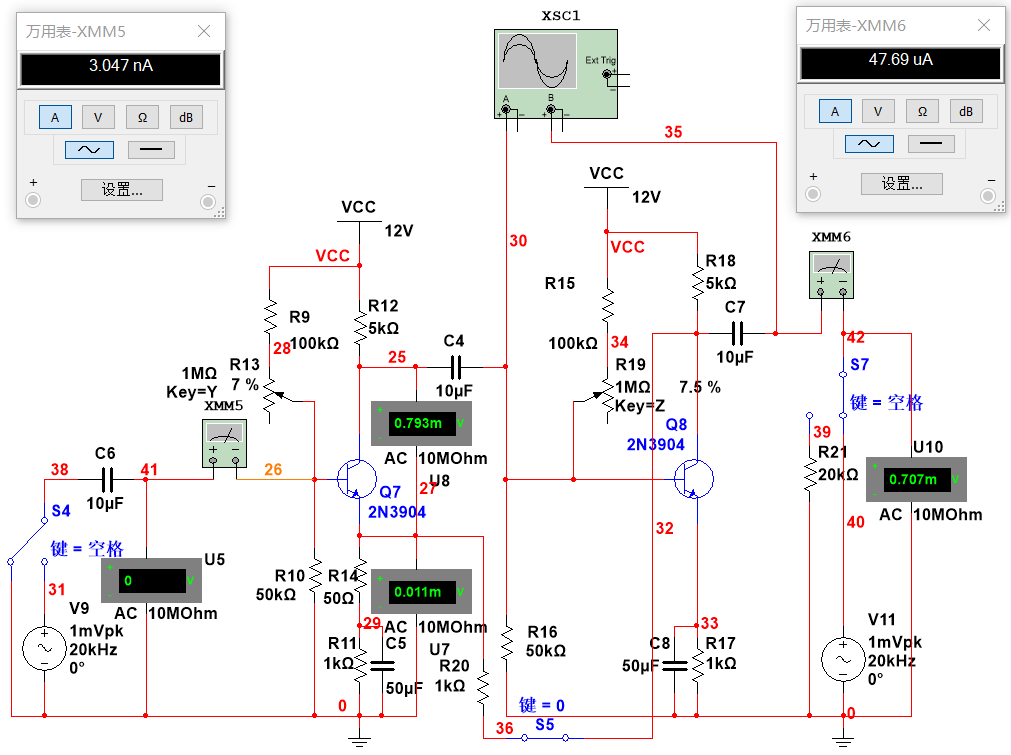
\includegraphics[width=\linewidth]{3/Ro-close.png}
		\caption{两级闭环放大电路输出电阻}
		\label{fig:两级闭环放大电路输出电阻}
	\end{subfigure}
	\caption{两级放大电路输出电阻}
	\label{fig:两级放大电路输出电阻}
\end{figure}

输出电阻测量原理图如图\subref{fig:两级闭环放大电路输出电阻}所示,即短路输入端电压源,断开负载电阻,并在输出端加入信号源。

采用交流分析法测量输出电阻,由图\subref{fig:两级开环放大电路输出电阻}可知无反馈时输出电阻为\SI{16.399}{\kohm}。

比较反馈接入前后输出电阻的变化可知电压串联负反馈减小了输出电阻,提高了负载功率。

\subsubsection{频率特性}%
\label{ssub:频率特性}

由图\ref{fig:两级开环放大电路}可知中频增益\SI{3664.781}{\dB},上下界频率响应对应增益为\SI{3663.781}{\dB},对应上界频率\SI{166.7390}{\kHz},下界频率\SI{97.4882}{\Hz}。

由图\ref{fig:两级闭环放大电路}可知中频增益\SI{21.216}{\dB},上下界频率响应对应增益为\SI{18.216}{\dB},对应上界频率\SI{27153.4}{\kHz},下界频率\SI{23.3005}{\Hz}。

由图\ref{fig:两级开环放大电路}、\ref{fig:两级闭环放大电路}对比可知,负反馈虽然减小了放大倍数,但展宽了通频带。

\begin{figure}[H]
	\centering
	\begin{subfigure}[H]{.8\linewidth}
		\centering
		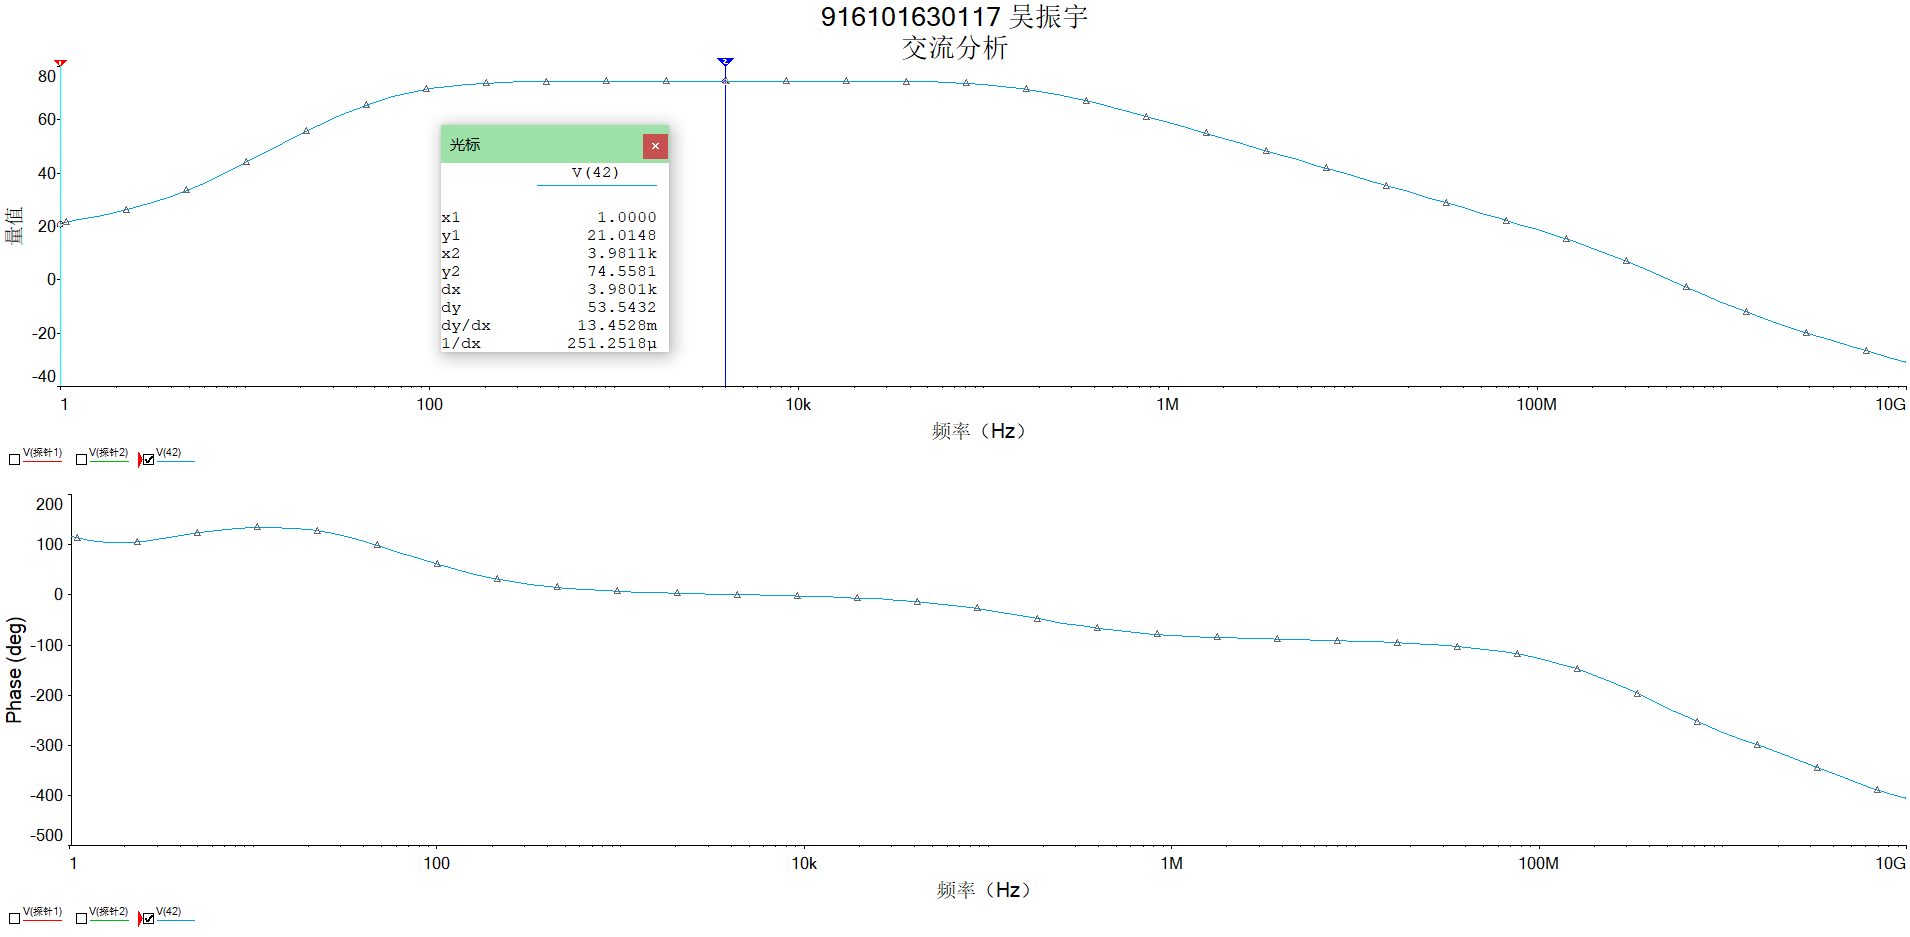
\includegraphics[width=\linewidth]{3/f-open.png}
		\caption{两级开环放大电路放大系数最高点}
		\label{fig:两级开环放大电路放大系数最高点}
	\end{subfigure}
	\quad
	\begin{subfigure}[H]{.8\linewidth}
		\centering
		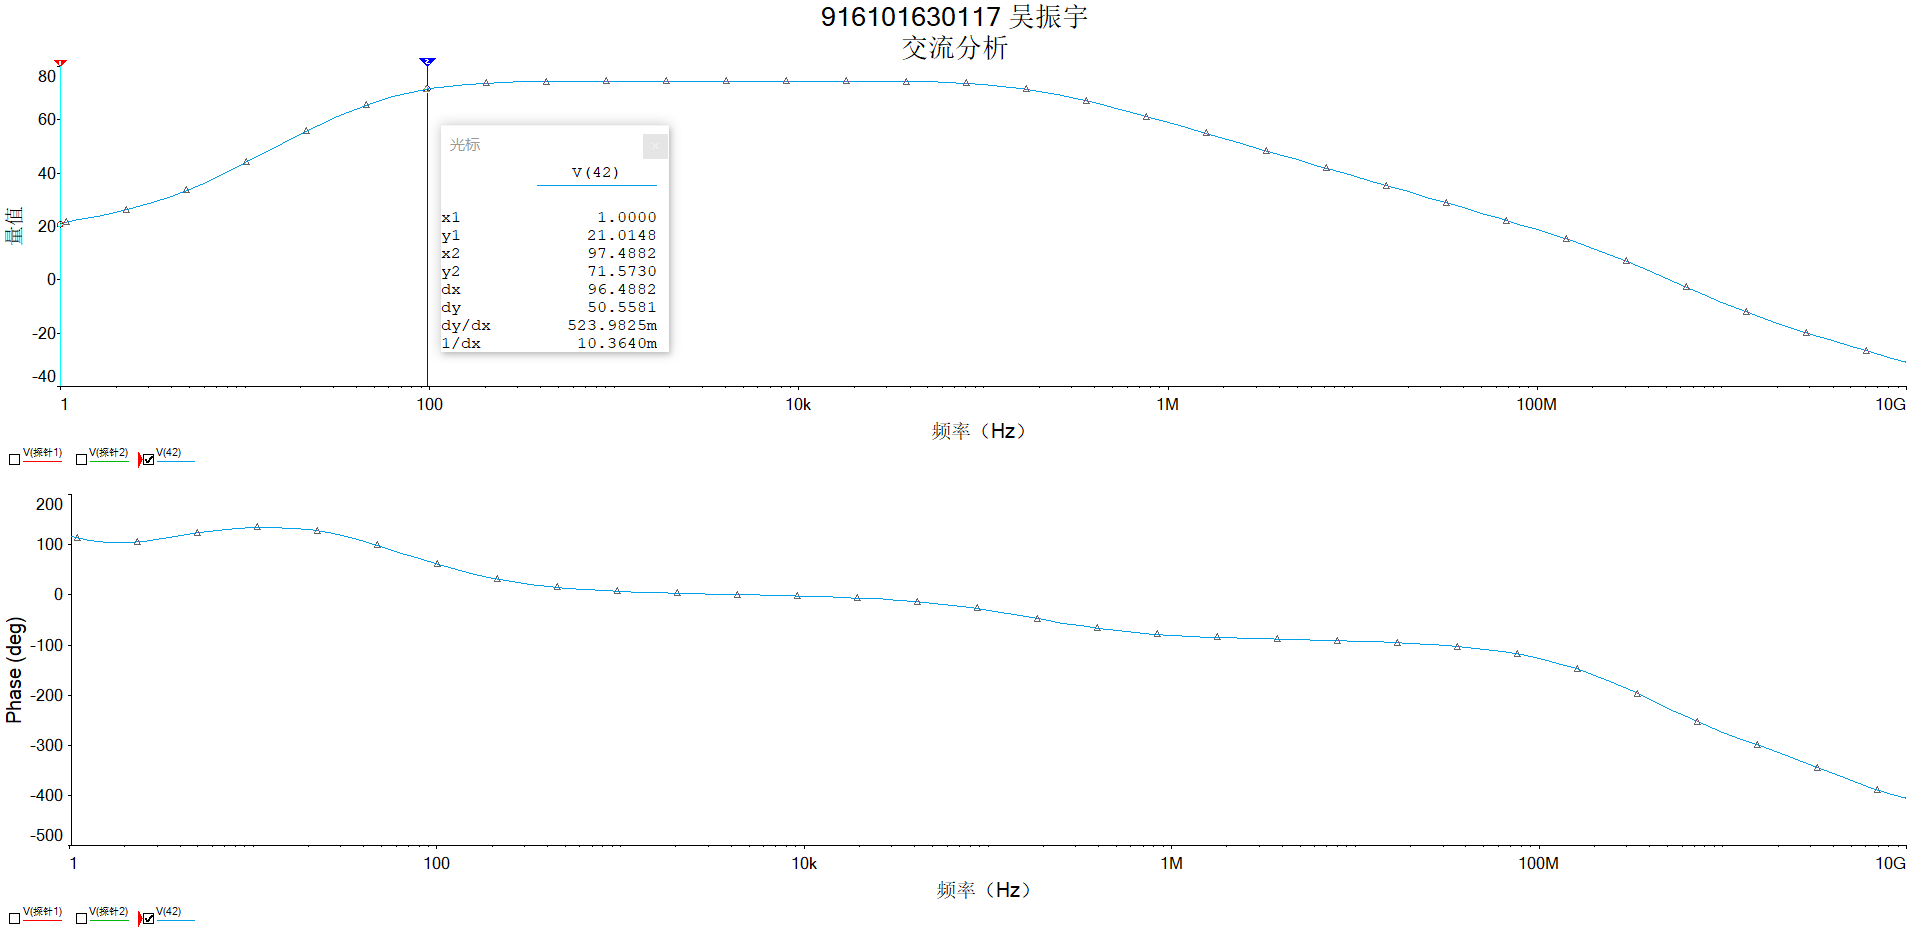
\includegraphics[width = 0.8\linewidth]{3/fL-open.png}
		\caption{两级开环放大电路下截止点}
		\label{fig:两级开环放大电路下截止点}
	\end{subfigure}
	\quad
	\begin{subfigure}[H]{.8\linewidth}
		\centering
		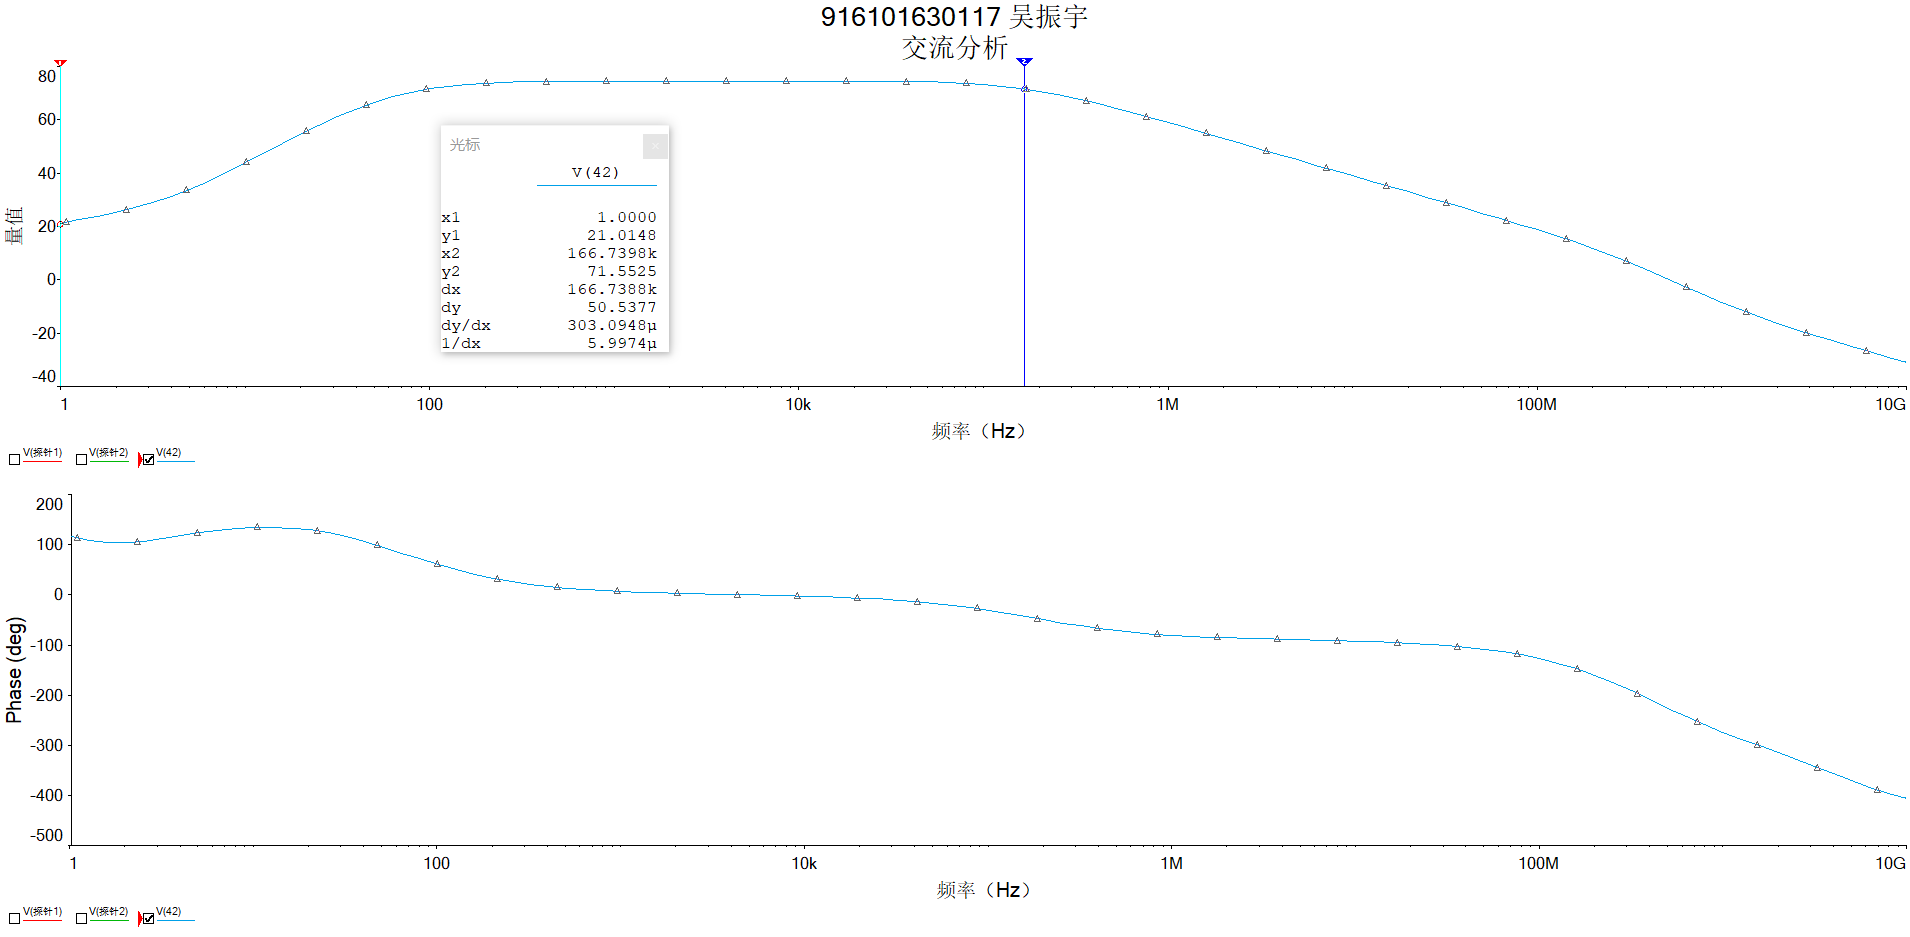
\includegraphics[width=\linewidth]{3/fH-open.png}
		\caption{两级开环放大电路上截止点}
		\label{fig:两级开环放大电路上截止点}
	\end{subfigure}
	\caption{两级开环放大电路}
	\label{fig:两级开环放大电路}
\end{figure}

\begin{figure}[H]
	\centering
	\begin{subfigure}[H]{.8\linewidth}
		\centering
		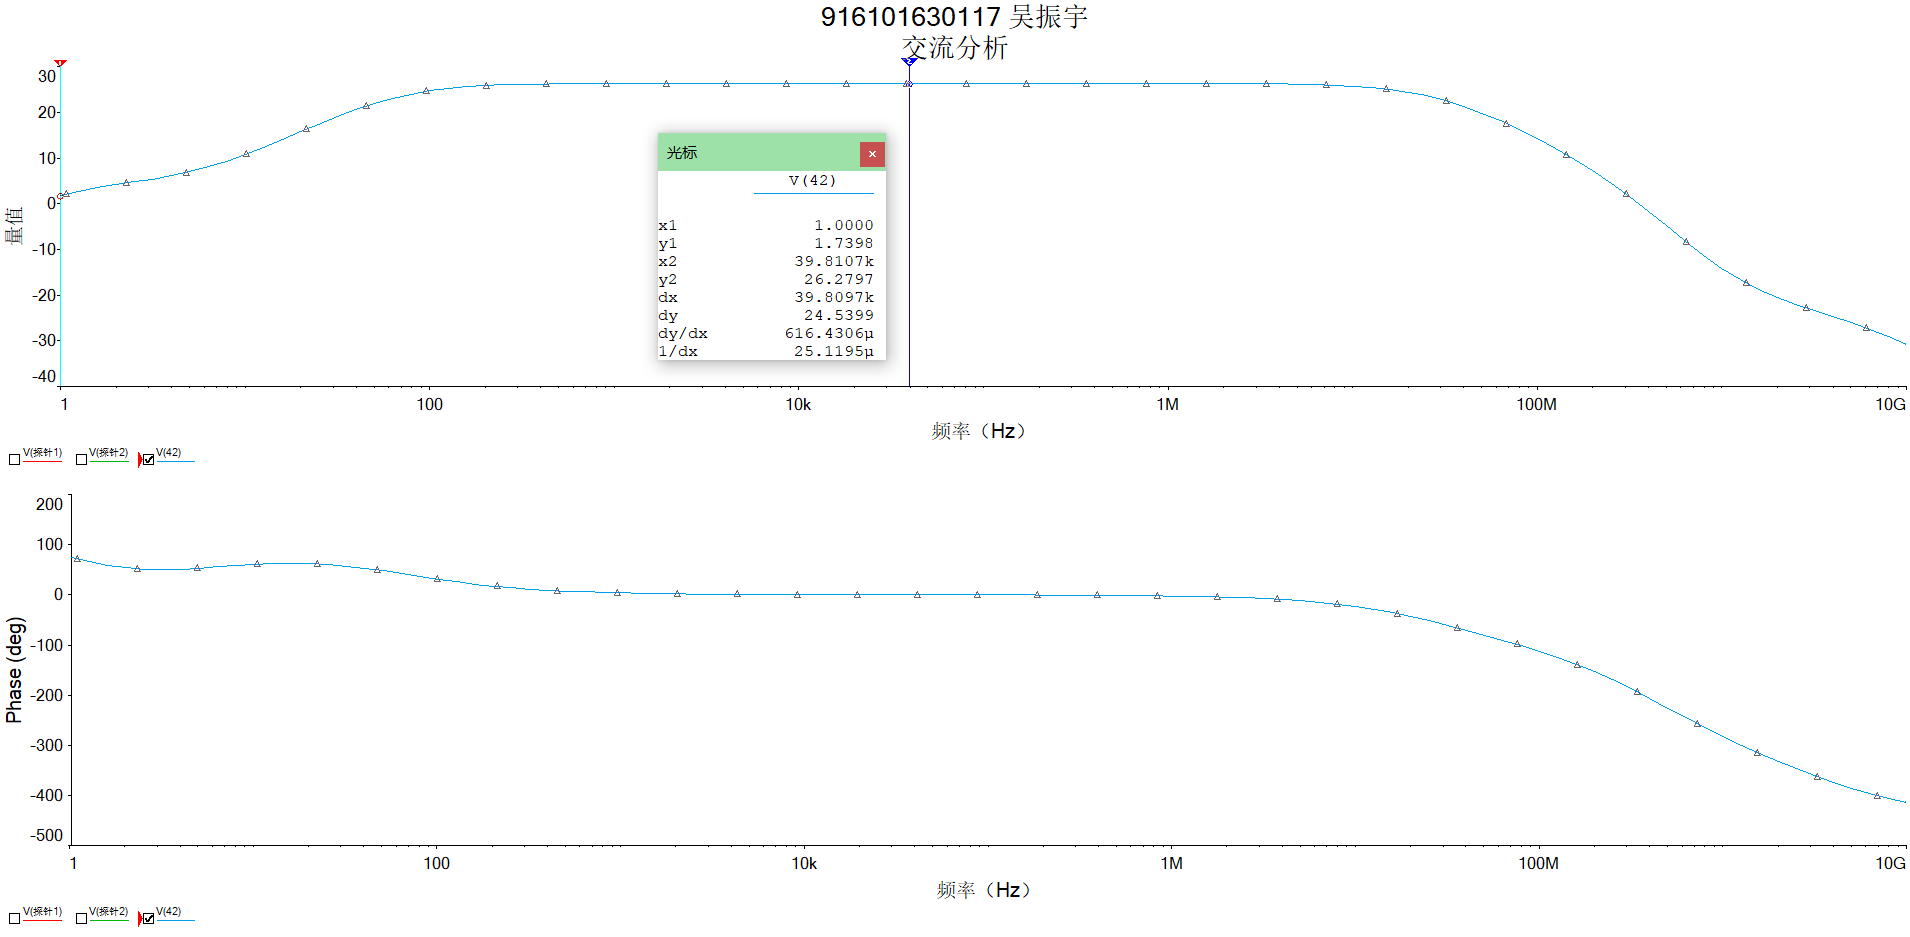
\includegraphics[width=\linewidth]{3/f-close.png}
		\caption{两级闭环放大电路放大系数最高点}
		\label{fig:两级闭环放大电路放大系数最高点}
	\end{subfigure}
	\quad
	\begin{subfigure}[H]{.8\linewidth}
		\centering
		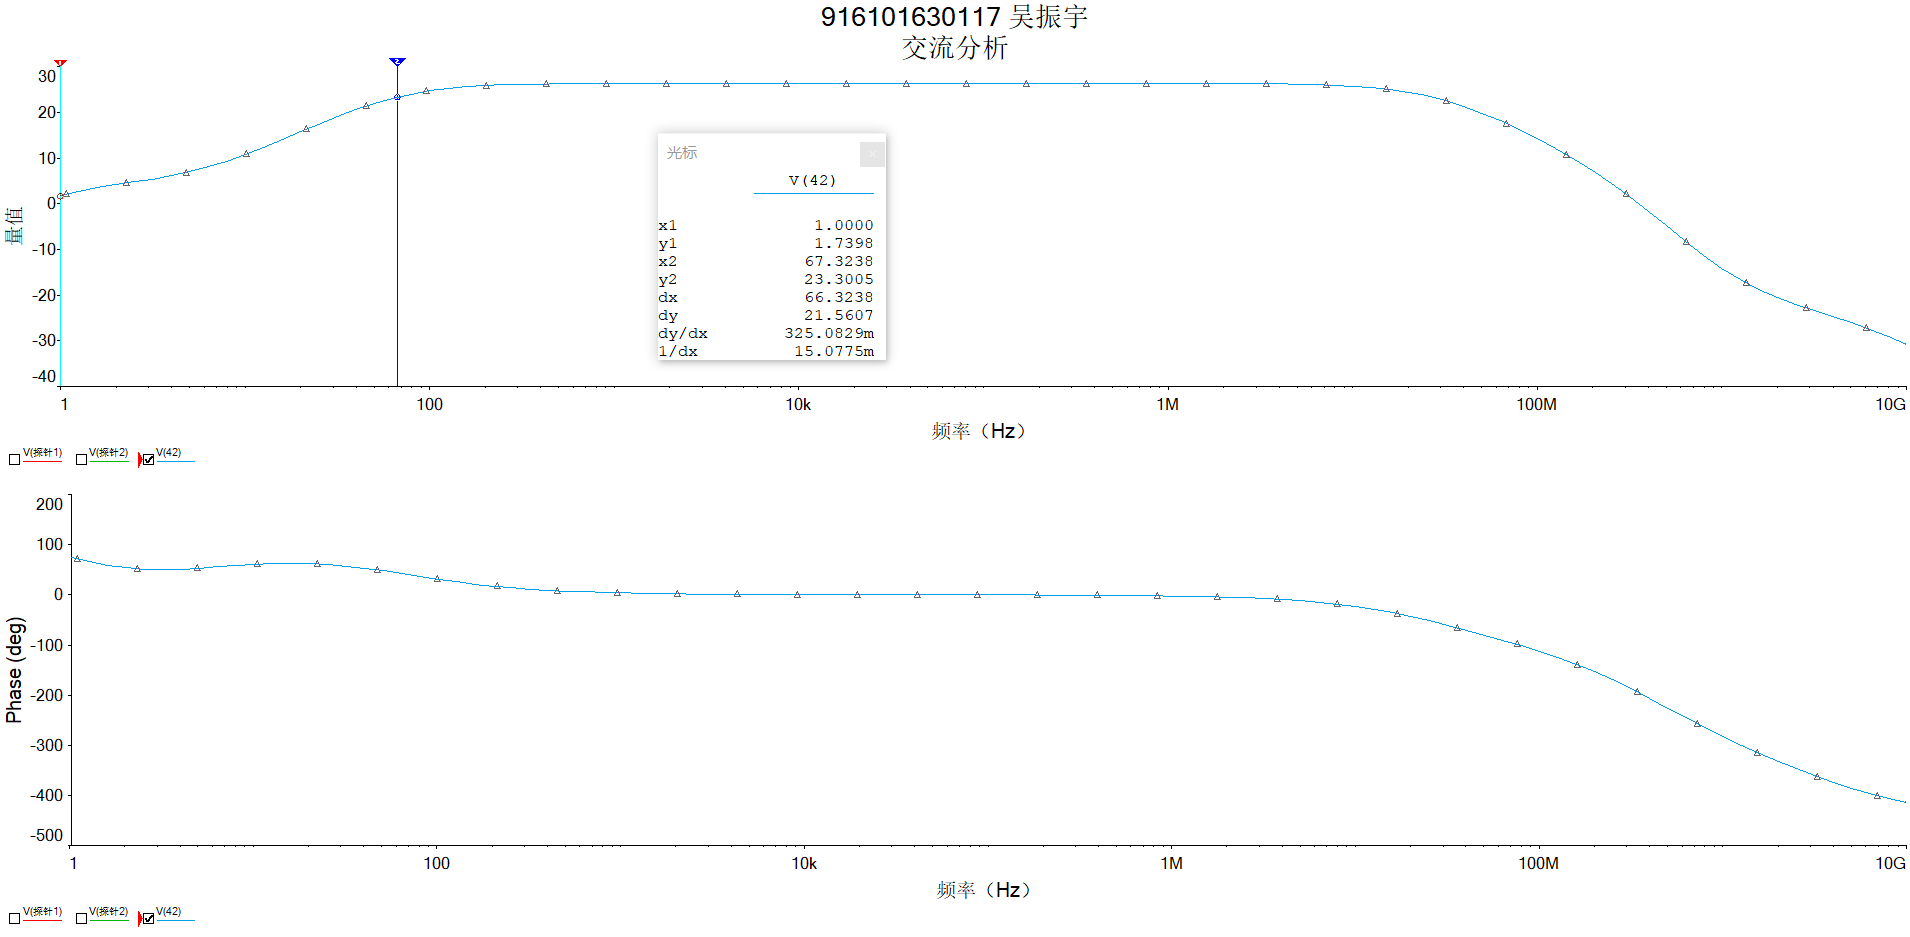
\includegraphics[width = 0.8\linewidth]{3/fL-close.png}
		\caption{两级闭环放大电路下截止点}
		\label{fig:两级闭环放大电路下截止点}
	\end{subfigure}
	\quad
	\begin{subfigure}[H]{.8\linewidth}
		\centering
		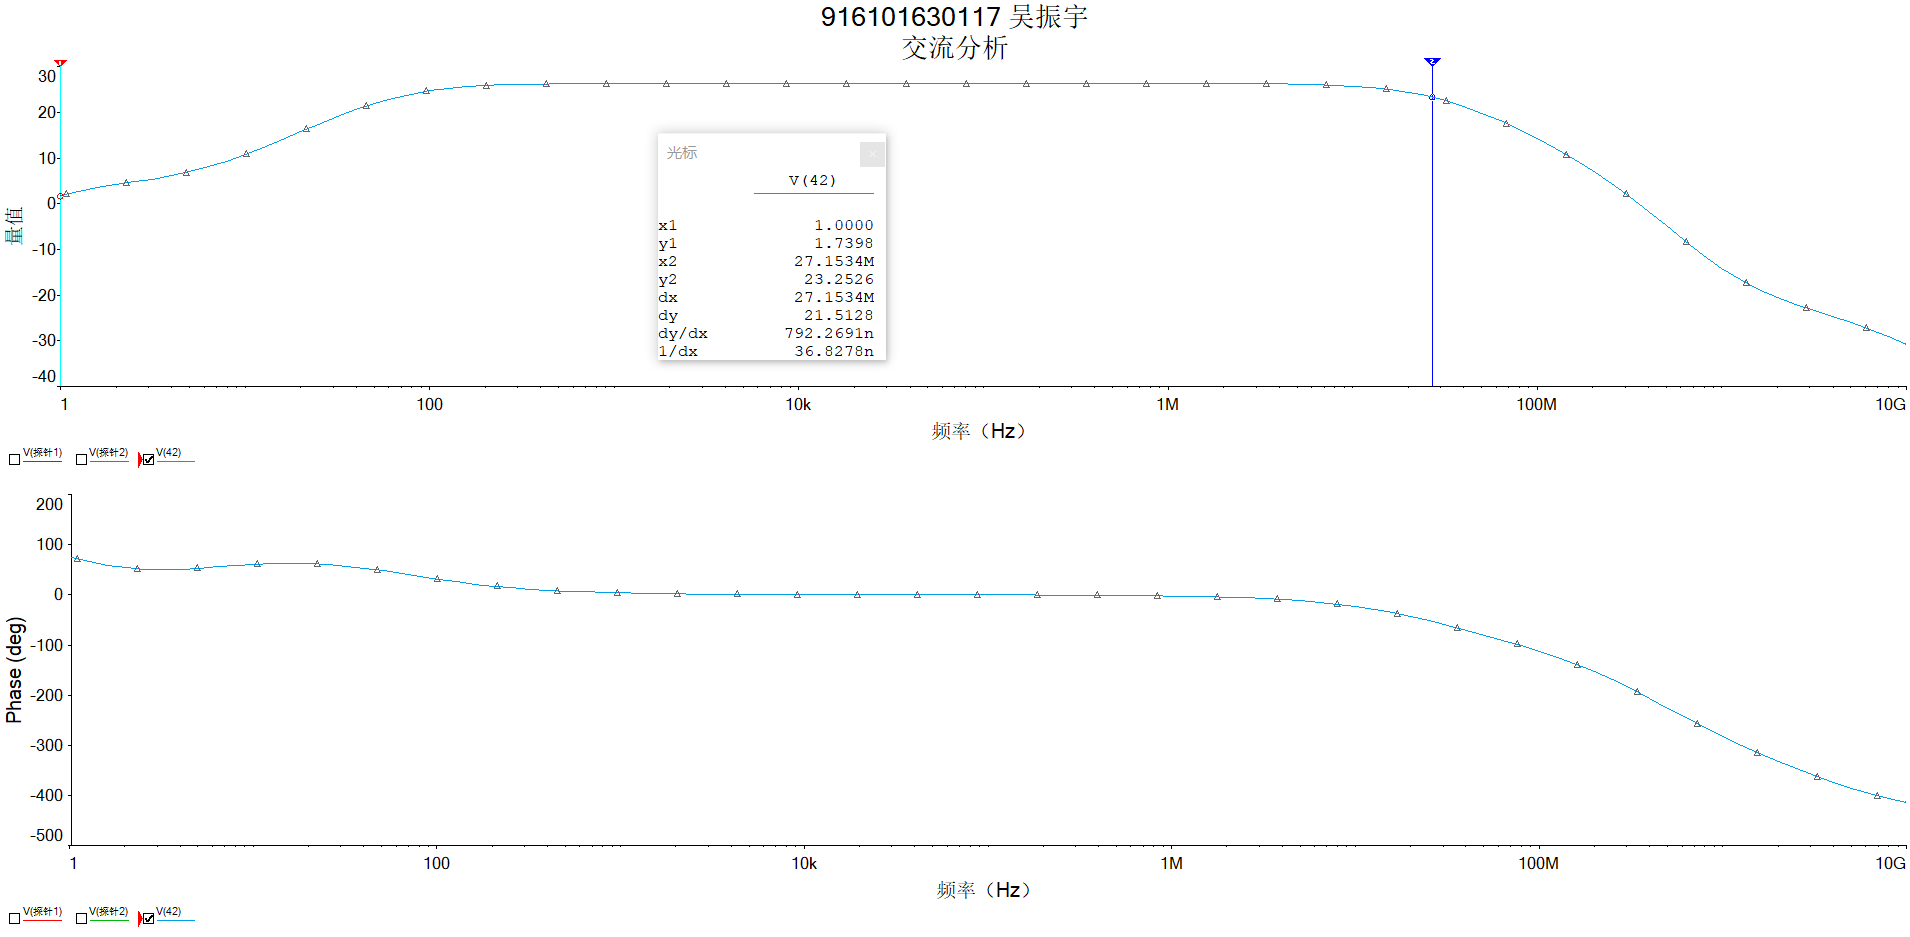
\includegraphics[width=\linewidth]{3/fH-close.png}
		\caption{两级闭环放大电路上截止点}
		\label{fig:两级闭环放大电路上截止点}
	\end{subfigure}
	\caption{两级闭环放大电路}
	\label{fig:两级闭环放大电路}
\end{figure}

\subsubsection{波形失真}%
\label{ssub:波形失真}

\begin{figure}[H]
	\centering
	\begin{subfigure}[H]{.7\linewidth}
		\centering
		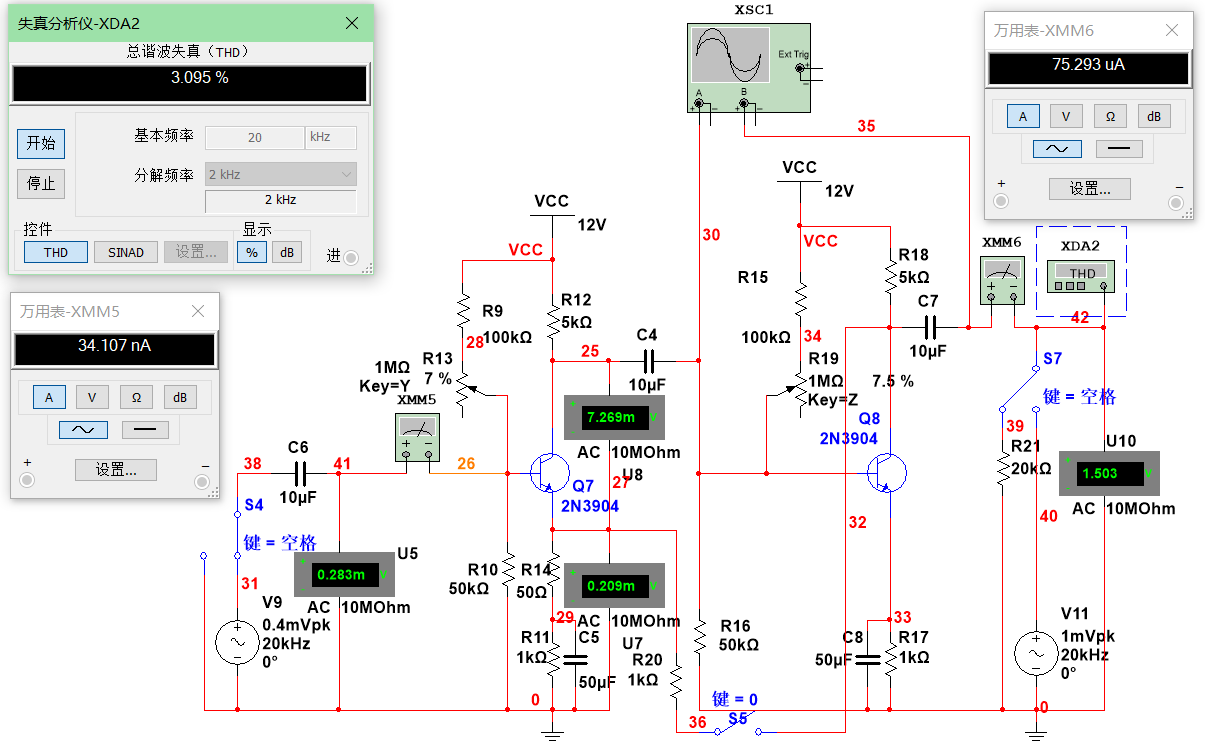
\includegraphics[width=\linewidth]{3/distortion-open.png}
		\caption{两级开环放大电路波形失真}
		\label{fig:两级开环放大电路波形失真}
	\end{subfigure}
	\quad
	\begin{subfigure}[H]{.7\linewidth}
		\centering
		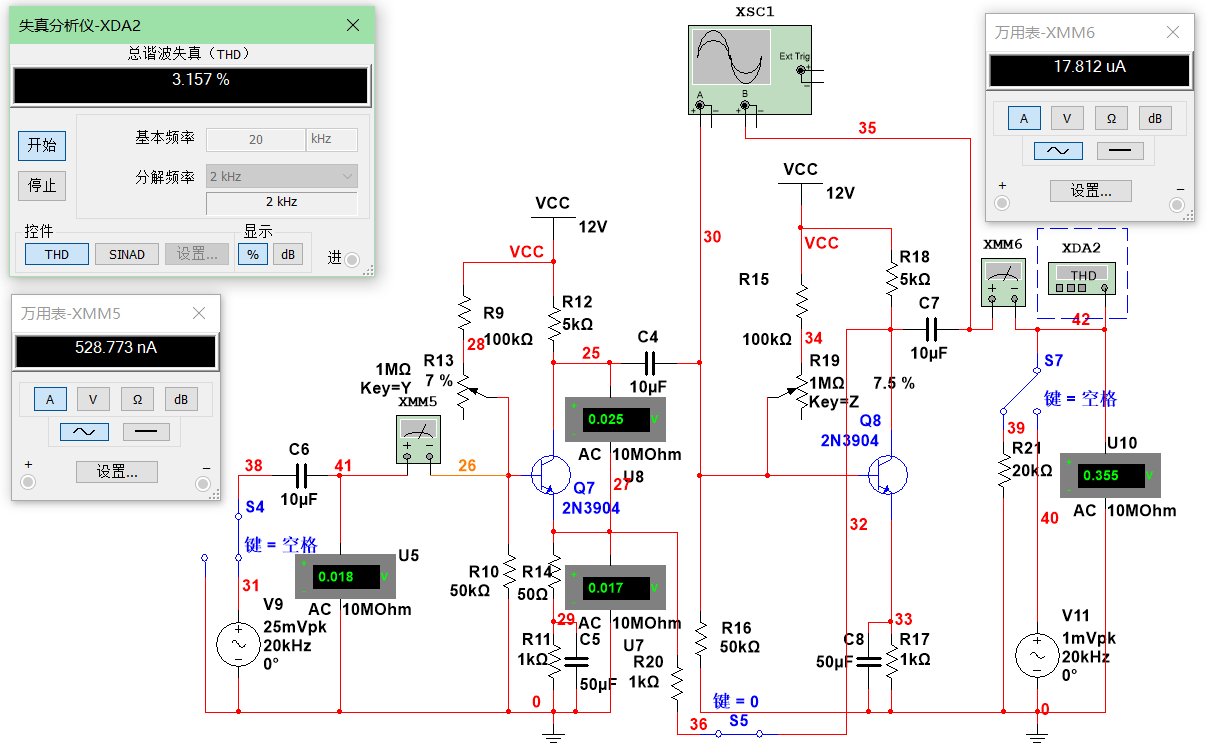
\includegraphics[width=\linewidth]{3/distortion-close.png}
		\caption{两级闭环放大电路波形失真}
		\label{fig:两级闭环放大电路波形失真}
	\end{subfigure}
	\caption{两级放大电路波形失真}
	\label{fig:两级放大电路波形失真}
\end{figure}

未接入反馈时如图\subref{fig:两级开环放大电路波形失真}所示,峰值为\SI{1}{\V}左右,正半周波峰略低于负半轴波峰,这是由于输出特性曲线中靠近截止区时曲线略有上移,而引起的非线性失真。

接入反馈时如图\subref{fig:两级闭环放大电路波形失真}所示,峰值为\SI{1}{\V}左右,正半周波峰几乎等于负半轴波峰,这是由于反馈网络的存在使$ X_\mathrm{i},X_\mathrm{f} $叠加后的输入量矫正了基本放大器的非线性失真。

由对比可知反馈网络对非线性失真具有改善作用。

\subsection{误差分析}%
\label{sub:\arabic{chapter}误差分析}

\subsubsection{放大倍数}%
\label{ssub:放大倍数}

有反馈情况下放大倍数约为21.216倍,反馈电阻值$ R_{20} = \SI{1}{\kohm} $,放大倍数理论值为$ 1 + \dfrac{R_{20}}{R_{14}} = 21 $,与实验结果相吻合。

\section{实验小结}%
\label{sec:\arabic{chapter}实验小结}

本次实验验证了$ A_\mathrm{F}\approx\dfrac{1}{F} $以及反馈电路对开环放大电路的影响。接入反馈电路后,放大倍数变小,电路的稳定性增加,带宽变宽,开始失真时的信号幅度变大。

